\documentclass[english]{lni}

\IfFileExists{latin1.sty}{\usepackage{latin1}}{\usepackage{isolatin1}}

\usepackage{graphicx}

\author{Alexander Gessler, Simon Hanna, Ashley Marie Smith\\Universit�t Stuttgart, Institute for Parallel and Distributed Systems \\ 
\{gessleah, hannasn, smithae\} @studi.informatik.uni-stuttgart.de}
\title{Scaling in a Distributed Spatial Cache Overlay\footnote{Based on a student project supervised by Carlos L\"{u}bbe at IPVS, University of Stuttgart}}

\begin{document}
\maketitle

\begin{abstract}
Location-based services for mobile devices are a type of distributed system which utilize geographic behavior of its users. 
Balancing dynamic query workloads and skewed data remains a problem. 
Scale-in and scale-out are two proposals that temporarily remove or add resources, respectively. 
To characterize situations where scaling is more efficient, 
we implemented a distributed spatial cache overlay for 2D data with the goal of evaluating system performance with and without scaling-out. 
In this paper, we present an experimental setup to benchmark such a system, 
and measurements of relative scalability under different cache overlay sizes, query rates and workload distributions. 
Our results indicate that the system achieves almost linear relative scalability for both uniform and non-uniform query distributions.
\end{abstract}

\section{Introduction}
Location-based services (LBS) are data-intensive applications which use the geographic behavior of the user in order to process queries. 
These queries access spatial data, which correspond to physical geographic regions. 
A typical example is a route-planning application for smartphones. 
The user sends an address as a query, and in response to the query, the application delivers data, 
which could be the corresponding portion of the map. 
A fundamental problem of LBS is how to allocate the workload in the system, 
so as to guarantee low latency and efficiency in processing these queries. 
Much research has focused on developing load-balancing mechanisms for distributed systems with spatial data.. 

However in an LBS, both data and query workloads have spatial and temporal aspects, 
which dynamically change and thus require special considerations. 
Query loads can vary depending on time or geographic density of users. 
For example, fewer queries are sent late at night or in rural areas. 
Sometimes many queries access data from one location, for instance when large crowds gather for an event. 
Moreover, the distribution of data can be skewed, i.e. non-uniformly clustered around certain spatial regions, like big cities. 

Given these spatial and temporal characteristics, 
we are interested in how to minimize decreases in system performance under such loads or data distribution. 
A common technique is to partition data and then build a network overlay, which dedicates nodes to handle requests for certain partitions 
\cite{p2p:godfrey} \cite{client:wee}. Some approaches then focus on reducing data skew via migration or replication of data, 
but at higher costs for storage \cite{migration:mondal}. 
Other approaches estimate query loads or calculate weights to place more nodes around expected hotspots \cite{grids:scholl}. 
Yet it is difficult to predict or respond to changes, such as moving hotspots. 
A more effective approach dedicates nodes in the overlay to cache frequently accessed data; 
this network is referred to as a \emph{distributed spatial cache overlay}. 

However, none of the previously mentioned load-balancing approaches in distributed spatial overlays 
can increase throughput beyond what is already the system maximum. 
Thus extreme spikes in query workloads can exceed the system's maximum capabilities. 
Adding and then removing additional resources to the LBS can address these temporary spikes. 
The idea is that the overlay automatically decides when to add or remove nodes, based on self-measured load. 
Adding nodes is referred to as \emph{scaling-in}, whereas removing nodes is referred to as \emph{scaling-out.}  
In the scope of our project, we investigate whether scaling-out mitigates dynamic peaks in a distributed spatial cache overlay. 

\section{Foundations}
Our system is based on \cite{disco:Luebbe}, \cite{MultiLevel:Lueb2}. 
The data region is partitioned into a 2D grid. 
Then a distributed cache overlay is built on top and consists of nodes dedicated to caching data from certain grid partitions. 
We refer to a cache node's coordinate as its \emph{cache focus}. 
The concept of cache focus is important during load-balancing and when nodes cache new data items. 
Suppose a node is serving a request but a local cache miss occurs. 
The cache node makes room in its cache list for the requested data by removing the entry with the greatest distance to its cache focus. 
Our grid of cache nodes forms a Delauney triangulation in a 2D metric space. 
Greedy routing is used to forward messages to the node that is closest to a certain coordinate. 

\section{Architecture and Methodology}
When designing our system architecture, as seen in figure \ref{arch}, 
we had to deliver a grid of cache nodes that are organized spatially and deployed on a cluster. 
These nodes can receive and forward queries.
The system is launched and shut-down by an external GUI but is independent thereof. 
The system runs remotely on a cluster of unspecified size and hardware 
and can test the grid under different load-balancing and scaling mechanisms. 
In addition to the given specifications, we included an administrative node, 
asynchronous communication between nodes, and a basic logging system. 
The administrative node only initializes the overlay construction. 

Our implementation of scaling-out relies on asynchronous message-passing and handshake confirmation between nodes. 
The basic idea is that when a node's workload exceeds a given threshold, then the node communicates with its neighbors, 
in order to confirm whether the overload could be releaved by the addition of a new node.

\begin{figure}[!ht]
  \begin{center}
    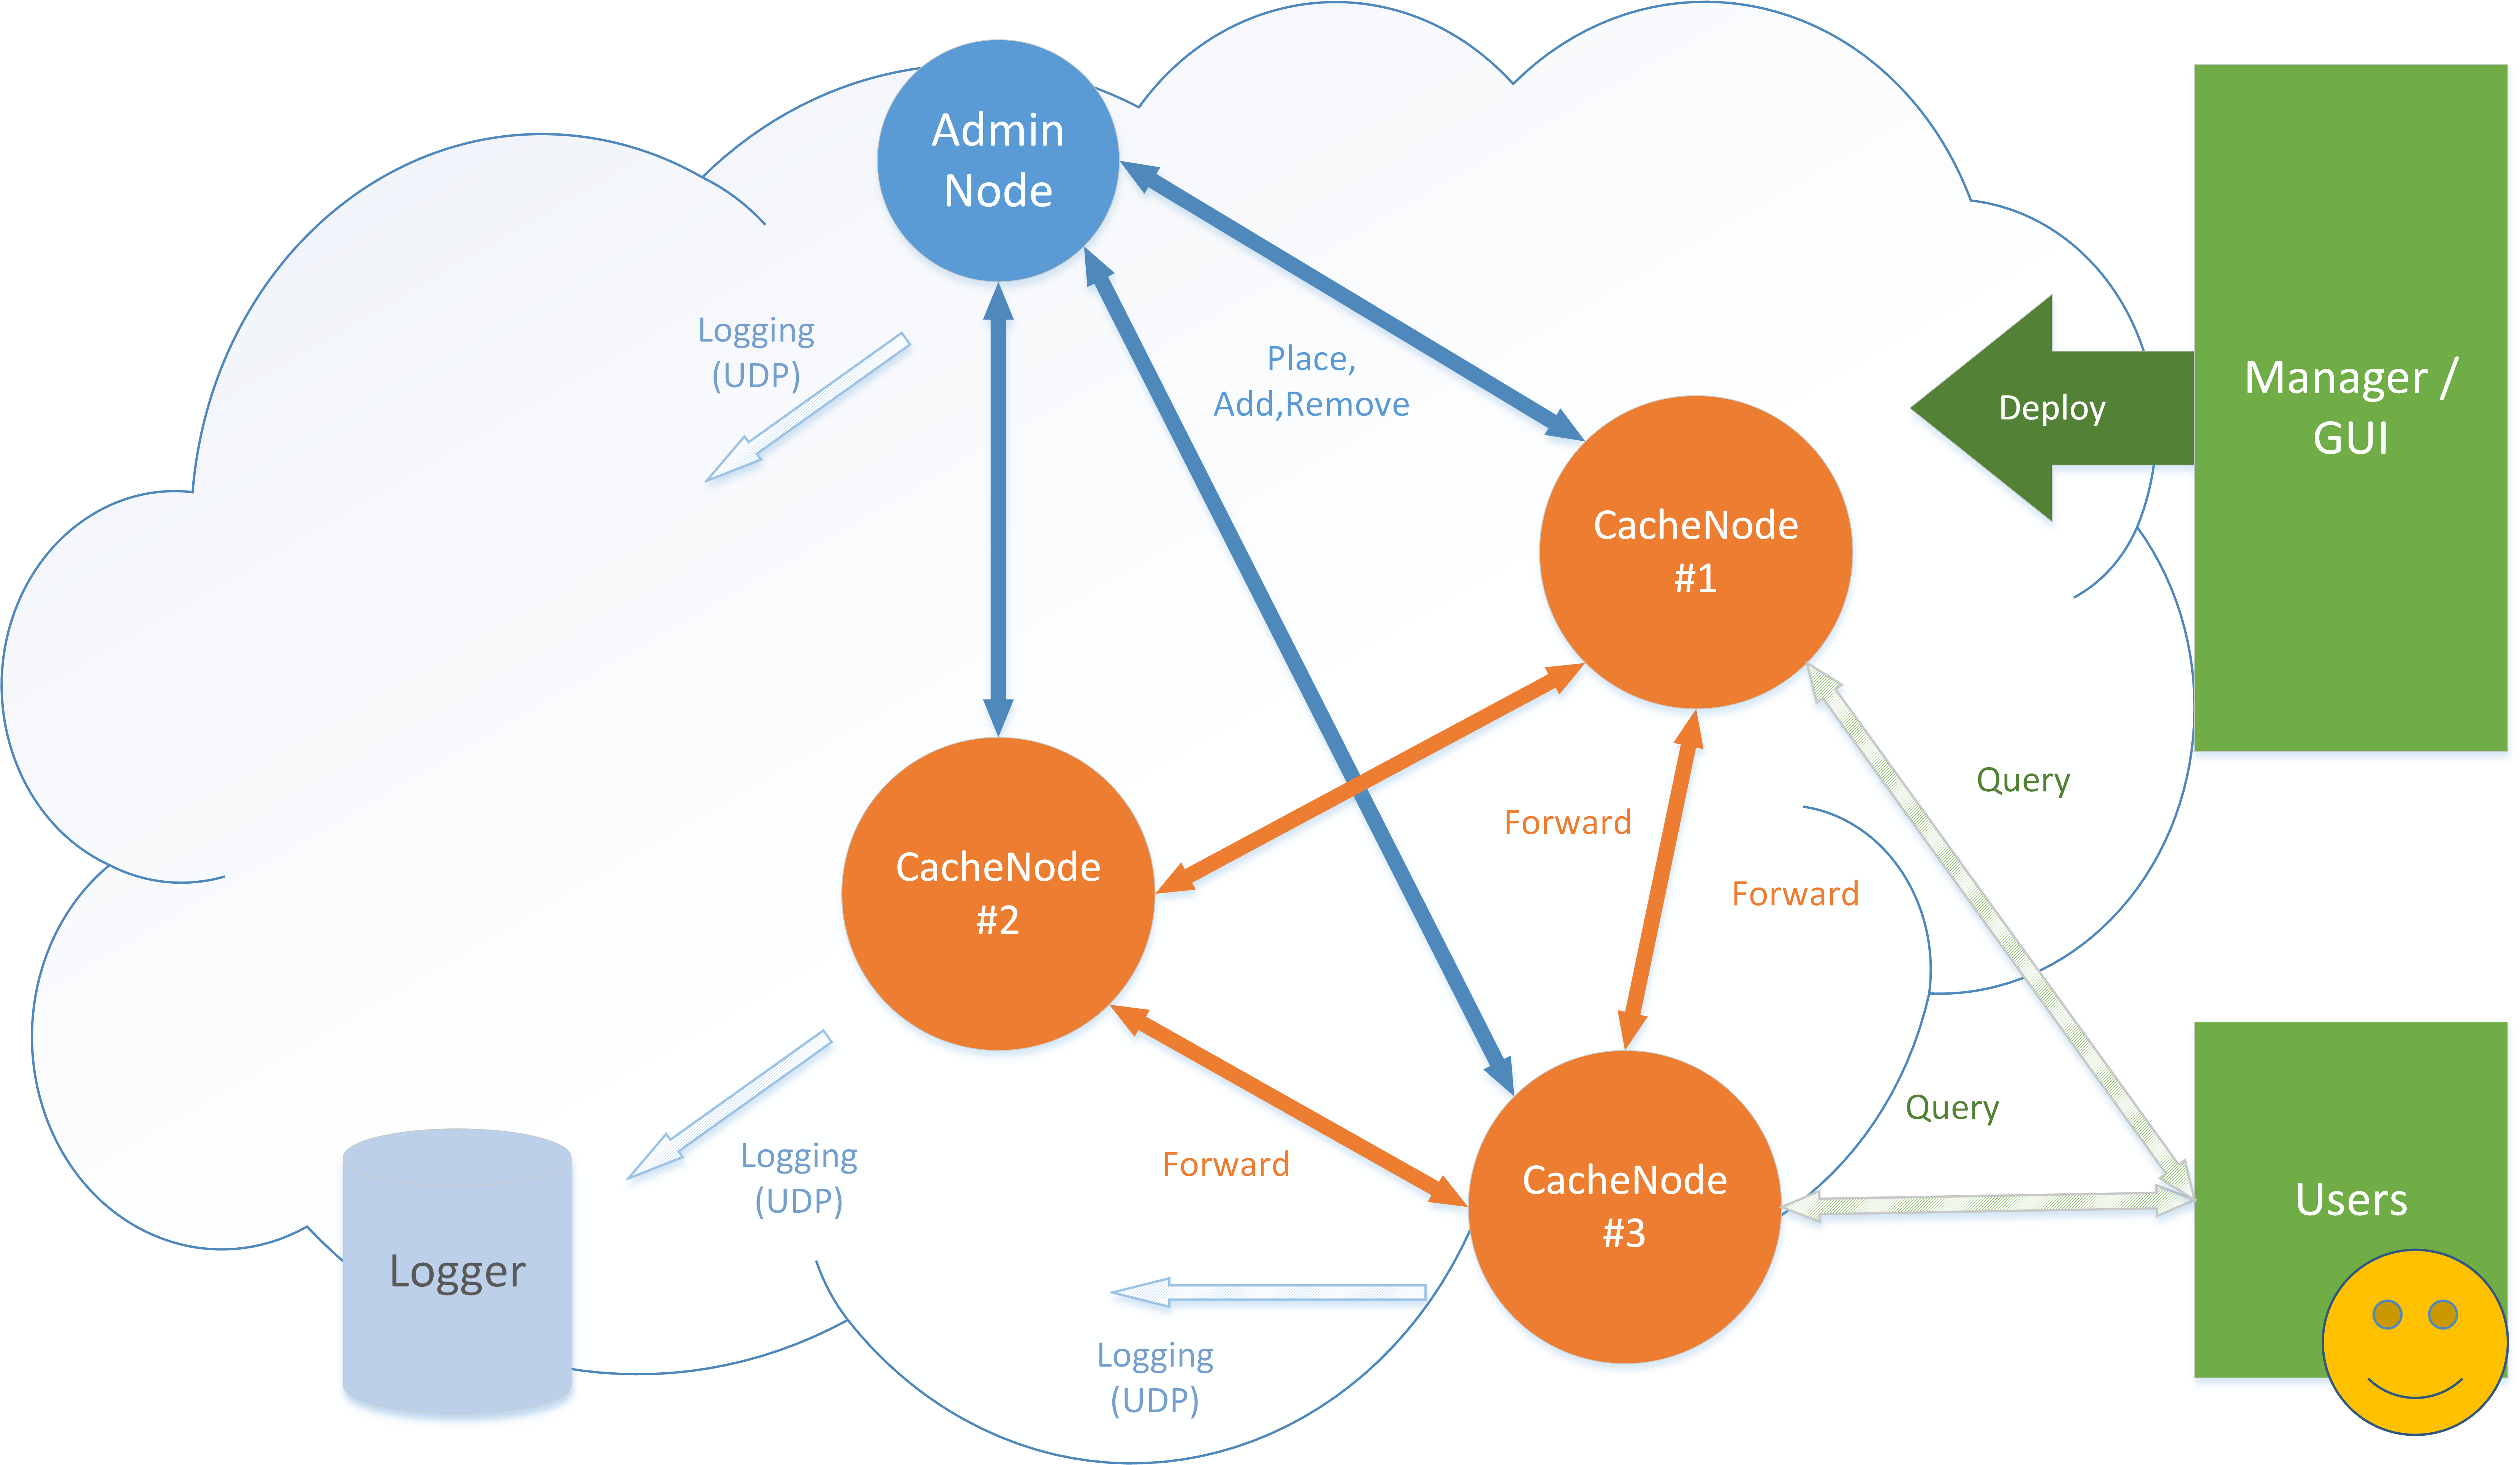
\includegraphics[width=\textwidth]{arch1}
    \caption{\label{arch}System Architecture of Cache as a Service}
  \end{center}
\end{figure}

The goal of our experiment was to quantify latency under uniform and non-uniform query loads.
In the uniform case, the target coordinates are distributed uniformly.
However in the non-uniform case, we can simulate the formation of hotspots: 
the target coordinate is obtained by sampling a Gaussian distribution 
with a standard deviation of 0.18 times the area of the data region that is centered around a point in the grid. 

We measured request latency of the cache overlay under four experimental groups: 
(1) under uniform queries with scaling-out, 
(2) under uniform query distribution without scaling-out, 
(3) under non-uniform query distributions with scaling-out, 
(4) under non-uniform query distribution without scaling-out. 

The distributed spatial cache overlay was launched on a cluster of up to 32 (virtual) machines. 
Our benchmarking program sent each cache node $k$ queries per second. 
This query rate corresponds to about $1000/k$ milliseconds between two successive queries. 
For every experimental group, we ran the benchmark program with query rates of $k = 15$ and $k=20$ 
and a given number of nodes ($n = 8, 12, 16$). 
Each run lasted $10$ seconds, so the total number of queries sent to the grid during each run was $n \cdot 10 \cdot k$. 

\section{Results and Discussion}
	For a given grid size $n$ and query rate $k$, figure \ref{results} shows the median latencies in milliseconds of all queries sent, 
	according to experimental group. The values for tests run under uniform distribution/without scaling-out are not shown. 
	They were, as expected, worse than uniform/scaling-out but better than hotspot/scaling-out and hotspot/without scaling-out. 
	The range of the axes differ: for the purpose of clearly showing median times when $k=15$, the axis ranges only from 0 to 140 $ms$. % BRAUCHEN WIR DIESEN SATZ?

  \begin{figure}[htb]
    \begin{center}
      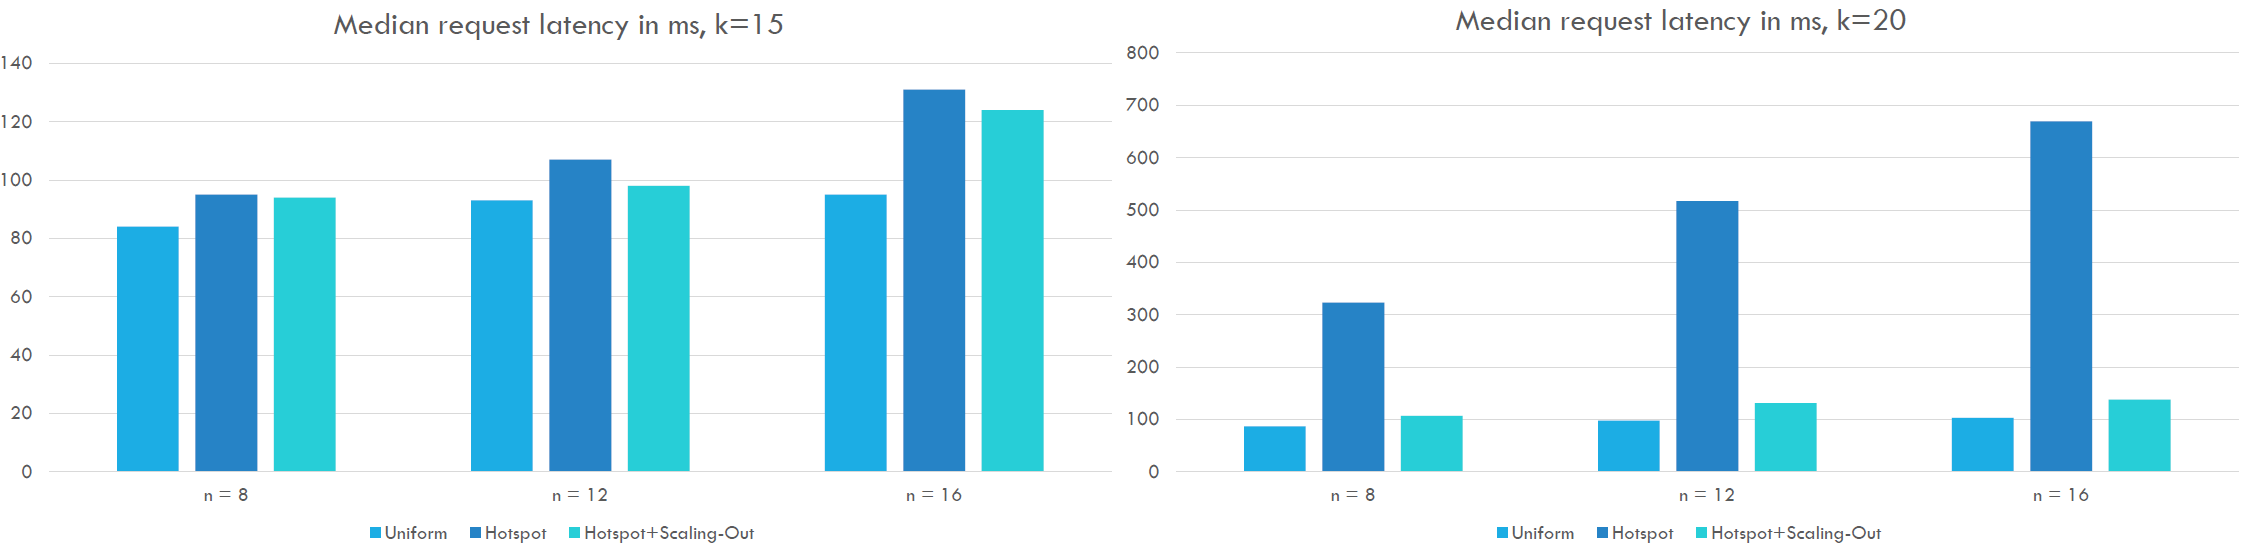
\includegraphics[width=\textwidth]{results}
       \caption{\label{results} Median Request Latencies}
     \end{center}
	\end{figure}

We hypothesized that with scaling-out, our system could approximate linear scalability, 
relative to resources, in both the uniform and non-uniform cases. 
Our results support our hypothesis. Under the higher request rate $k=20$, 
latency increases markedly for the non-uniform (no scaling-out) group. 
In contrast, the median times for the non-uniform(scaling-out) group when $n=16$ remain within 30 percent of the median latencies 
when $n=8$, although the total number of nodes has doubled and therefore the amount of queries being routed to the hotspot has also doubled.
			
\section{Conclusion and future work}
In our study, we designed, implemented and evaluated a distributed spatial cache overlay 
that is flexible enough to allow implementations of more sophisticated load-balancing schemes. 
This cache overlay serves as the basis for further comparisons of various load-balancing mechanisms 
to see whether linear scalability relative to resources can be achieved. 
We confirmed that non-uniform workloads cause the system's performance and scalability to degrade under higher query rates. 
We also showed that even with non-uniform workloads, 
the system with scaling-out is able to scale almost linearly relative to resources. 
Our preliminary results justify further evaluation of the system.

Based on our preliminary results, our primary focus will be to implement scaling-in and elastic load-balancing 
to handle changes in both global and relative load. 
Since our current implementation exhibits a routing time of $\mathcal O (\sqrt{n})$, 
we propose maintaining connections to nodes that are not directly connected. 
This should drop the routing time to $\mathcal O(log(n))$.

\bibliography{lniguide}

\begin{thebibliography}{1}

\bibitem{migration:mondal}
A.~Mondal, et al. 
``Effective Load-balancing via Migration and Replication in Spatial Grids."\\
\emph{Dexa, Vol. 2736}: Springer, 2003: pp.202-211. \\

\bibitem{p2p:godfrey}
B.~Godfrey, et al. 
``Load Balancing in Dynamic Structured P2P Systems."\\
\emph{23. INFOCOM}: IEEE Computer Society, 2004. \\

\bibitem{grids:scholl}
T.~Scholl, et al. 
``Workload-Aware Data Partitioning in Community-Driven Data Grids."\\
\emph{EDBT}: ACM, 2009.\\

\bibitem{MultiLevel:Lueb2}
C.~L\"{u}bbe, et al. 
``Holistic load-balancing in a distributed spatial cache."\\
\emph{MDM}: IEEE Computer Society, 2013: pp. 267-270.\\

\bibitem{disco:Luebbe}
C.~L\"{u}bbe, et al. 
``DiSCO: A Distributed Semantic Cache Overlay for Location-Based Services."\\
\emph{MDM}: IEEE Computer Society, 2011: pp. 1-10.\\

\bibitem{client:wee}
S.~Wee and H.~Liu. 
``Client-side load balancer using cloud."\\ 
\emph{SAC}: IEEE Computer Society, 2010, pp. 399-405.\\

\end{thebibliography}




\end{document}

